\chapter{Conclusion and Future Scope}
\label{conclusion}

\section{Sci-Genie: Technical Debts and Shortcomings}
Although Sci-Genie provides a more context rich access to search results, the components that help enrich context during search i.e., the parsing/indexing can be further improved. This section details the limitations of some components. Based on some of these limitations, future work is described in Section \ref{conclusion:future-scope}.

\subsection{Heuristic Parsing}
\begin{figure}[h]
    \centering
    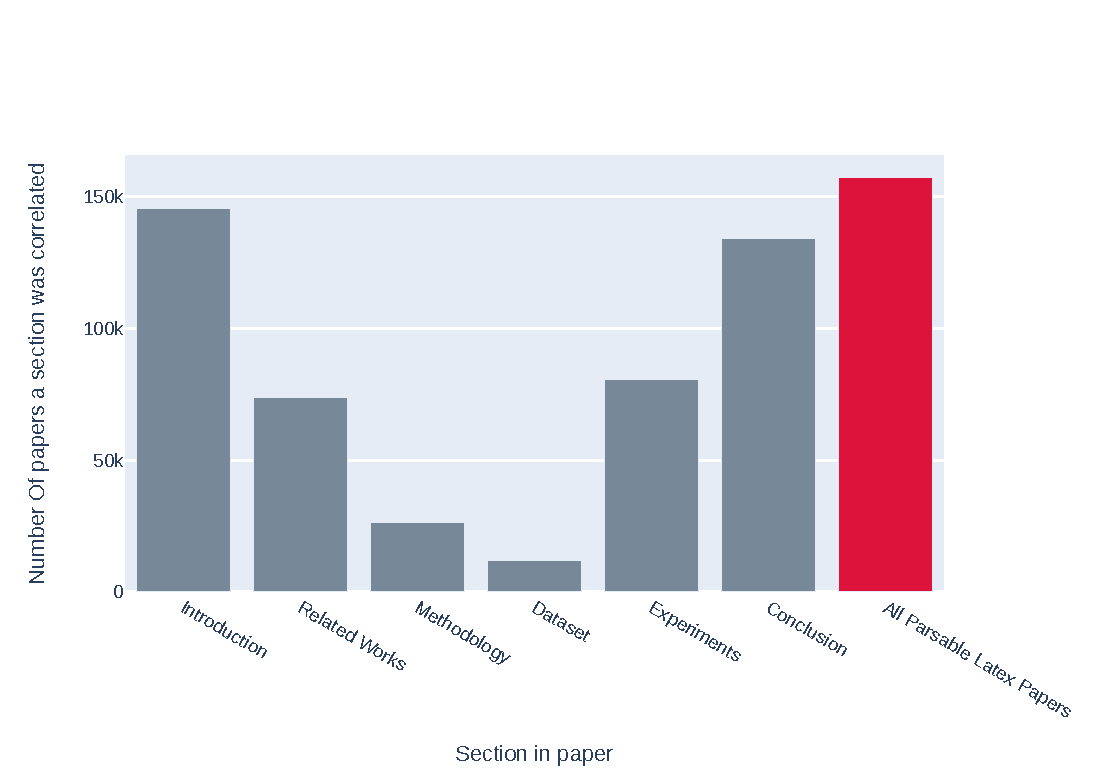
\includegraphics[width=\maxwidth{\textwidth}]{src/images/parsing-stats.pdf}
    \caption{ A bar plot of number of documents where a section got parsed by the heuristic parser from 158K papers. }
    \label{figure\arabic{figurecounter}}
\end{figure}
\refstepcounter{figurecounter}
Sci-Genie uses a heuristic parser for parsing research documents. The heuristic parser correlates the Fragment object to the appropriate keys in the \nameref{sci-genie-core:data-layer:researchobj}. Figure \ref{figure21} shows the statistics of parsing using the heuristic parser from a total corpus of 158K papers. As the parser misses out many sections it can be further improved using better methods. The parser also considers the sections based on ones observed in CS papers. Future research directions can include identifying common patterns in the structure of research documents for fields outside CS; Research directions can include identifying domain specific document structural patterns to create a taxonomy that can be used as a part of parsing.


\subsection{CS ArXiv Only Access \& No Specialized Ranking}
While ArXiv can be a source of freely available well cited research, it also remains a preprint server where lots documents are not gauranteed to be cited. As Sci-Genie doesn't use citations or any other indicator as a metric for ranking search results, it lacks providing most well cited information. Sci-Genie is also specialized to CS and its ontology classifier uses CS specific domains. 

Future versions can extend the search engine to support more fields of research and use ontology for those fields. Future versions can even include better ranking schemes for the documents.  

\section{Future Research Scope}
\label{conclusion:future-scope}
\subsection{Grannular Table Type Classification}
\label{conclusion:future-scope:type-class}

The table types defined by \cite{kim2012scientific} are general purpose descriptions which can apply to various domains. Although they are quite useful, tables in recent CS literature have more grannular sub-classifications. For example a "Statistics Table" could be describing a Dataset for Machine Learning experiments. The tables which may seem as Experiments Results can also be describing an Ablation Study conducted on a ML model. Due to a very nuanced distinction between a lot of these tables, The task of machine learning to classify table types needs more grannular sub-types within the classes defined by \cite{kim2012scientific}. 

Multiple grannular table types such as Ablation Study, Dataset Descriptions, can also be further described based on the field of research the tables belong to. The interface shown in Figure \ref{figure17}, was developed to annotated tables from scientific research. This interface can be extended for many fields outside CS; This inturn can aid the effort of curation and indentification of various types of tables from different avenues of research. 

\subsection{Discovering Related Tables}
\begin{figure}[h]
    \centering
    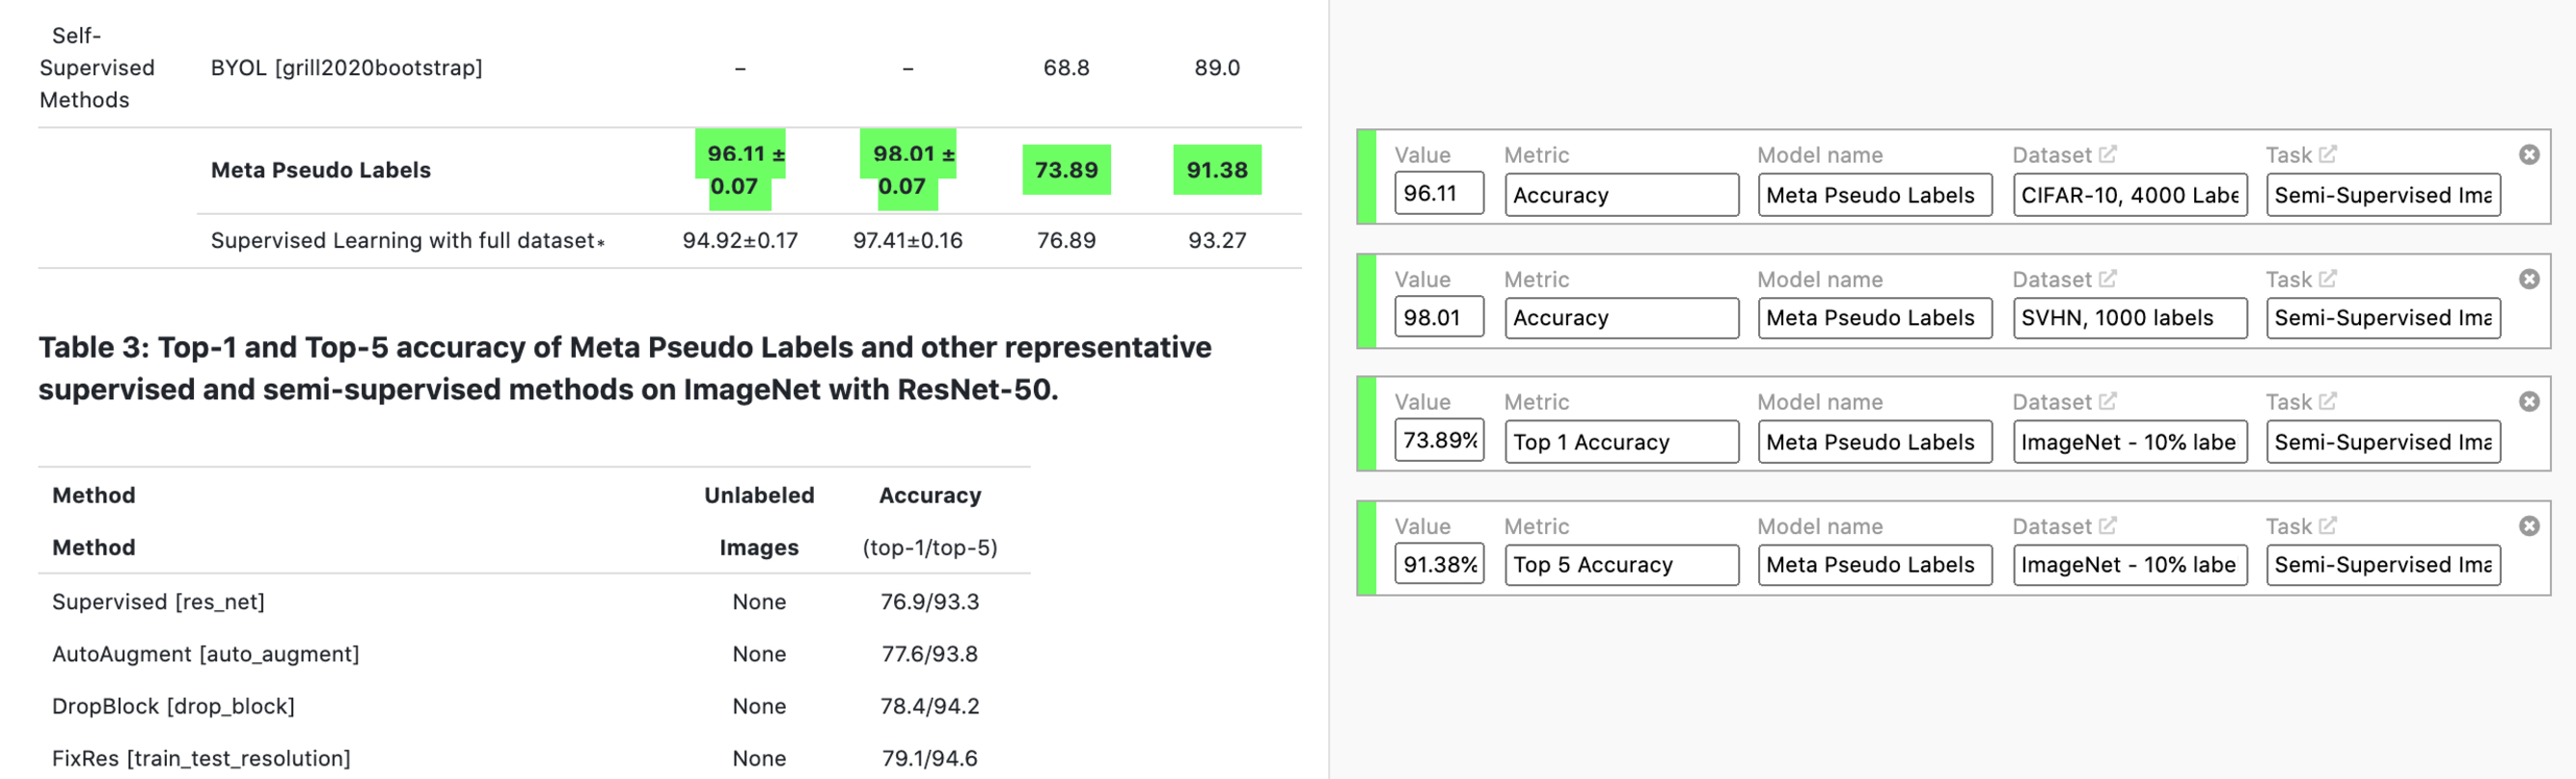
\includegraphics[width=\maxwidth{\textwidth}]{src/images/pwc-table-exp.pdf}
    \caption{ Viewing Tables For State of the art benchmarks using https://paperswithcode.com. }
    \label{figure\arabic{figurecounter}}
\end{figure}
\refstepcounter{figurecounter}
Organisations such as PapersWithCode(PwC) have developed tools to correlate information about SOTA ML methods from papers on ArXiv. PwC parses LaTeX based tables and correlates the benchamark metrics manually or via the use of libraries like AxCell\footnote{https://github.com/paperswithcode/axcell}. 

The benchmark correlation methods used by PwC are specific to ML SOTA benchmarks, Future research directions can include the automated extraction, corellation, and storage of tables from research papers into strict relational databases for domains outside ML and CS. 

\subsection{Scientific Research Document Parsing For Search Context}
Google search pivoted to ranking results for search using BERT\footnote{https://blog.google/products/search/search-language-understanding-bert/} since 2019. The trend of using language models to help rank search results has lead to creation of opensource tools\footnote{https://github.com/deepset-ai/haystack} that rerank documents over off the shelf search engines like Elasticsearch. But search ranking alone would not solve the search context problem as described in Chapter \ref{section:intro:missing_traits}.

Intelligent parsing maybe one part of the solution. Sci-Genie are uses domain specific content parser which is heuristically derived (Chapter \ref{sci-genie-core:scraping:frag-to-rs}) to help bring context relevant information in search results. This parser may not be applicable to other domains or document types.

\cite{kashyap2020sciwing}, introduced deep learning based techniques for scientific document parsing. \cite{kashyap2020sciwing}'s model generates a general purpose parsing structure. Although very useful, Every domain's document parse structure also have domain specific characteristics; For example, papers in Machine Learning explicitly have sections describing datasets in the paper. Identifying such patterns for generate domain specific parse structures for indexing can be a useful future direction of research for improving search context in academic search.

\section{Conclusion}
The fast rate of growth in technological progress will dramatically increase the growth in the volume of research in the future. Figure \ref{figure1}, is the best proof of that insight. The growing volume of research would also require more nuanced search tools which can help surface enough context around search terms and futher aid the researcher when reading research. This dissertation described a search engine and browser app based prototype solution to help remediate this problem. This dissertation covered the formulation of different aspects of the search engine and the ML models powering its table of comparison filtering algorithm. 

In summary, the proposed solutions in this dissertation try to remediate the problem of growth in the volume of research by aiding the researcher with more context based information when searching for research and reading research.